%%%%%%%%%%%%%%%%%%%%%%%%%%%%%%%%%%%%%%%%%%%%%%%%%%%%%%%%%%%%%%%%%%%
%%%%%%%%%%%%%%%%%%%%%%%%%%%%%%%%%%%%%%%%%%%%%%%%%%%%%%%%%%%%%%%%%%%%
\section{Comparing Inverse Problems and Solutions}\label{sec:compare}
%%%%%%%%%%%%%%%%%%%%%%%%%%%%%%%%%%%%%%%%%%%%%%%%%%%%%%%%%%%%%%%%%%%%
%%%%%%%%%%%%%%%%%%%%%%%%%%%%%%%%%%%%%%%%%%%%%%%%%%%%%%%%%%%%%%%%%%%%%%%%%%%%

As discussed in the introduction, the typical Bayesian approach to an inverse problem focuses on first modeling epistemic uncertainties in data on a QoI obtained from a true, but unknown, parameter value, which we denote by $\paramref$.
This is in contrast to the SIP and its observation-consistent solutions that are defined as pullback measures of an observed probability measure on the QoI.
To help build intuition about these differences, we summarize key details about these inverse problems and their solutions before presenting an example that highlights differences in solutions.

%As mentioned in the introduction, the observation-consistent framework developed in \cite{BJW18a, BJW18b, BWY20} is designed to quantify aleatoric sources of uncertainty while the typical Bayesian framework \cite{0266-5611-7-5-003,
%  Kennedy_O_JRSSSB_2001,Tarantola_book, MNR07, CDS10,starktenorio,
%  AlexanderianPetraStadlerEtAl14, Bui-ThanhGhattas14, Ernst2014,
%  0266-5611-30-11-110301, ROM:CMW_2016,Stuart10,
%  cockayneoatessullivangirolami} is designed to quantify epistemic sources of uncertainty.
%These conceptual differences have significant impacts on the solutions to inverse problems formulated within these distinctive frameworks.
%We provide more details below to further clarify these impacts for the reader.
%An example is then used to illustrate the differences, which is also helpful for building intuition.
%Moreover, the details provided below play a vital role in Section~\ref{sec:estimation} where features of the observation-consistent framework are used to motivate its extension to point estimation problems.


%The Bayesian inversion framework  is perhaps the most
%popular approach in the UQ community for incorporating uncertainties in inverse solutions.
%As discussed in the introduction, the typical Bayesian framework focuses on first modeling epistemic uncertainties in data on a QoI obtained from a true, but unknown, parameter value, which we denote by $\paramref$.

\subsection{Terminology, notation, and the inverse problems}

To make comparisons more clear, we first introduce shared notation between the SIP and Bayesian inverse problems.
Denote by $\pspace$ the space of physically relevant parameters for the model.
Denote by $Q$ the (potentially vector-valued) QoI map from the parameter space, $\pspace$, to the data space defined by $\dspace:= Q(\pspace)$.

\subsubsection{The stochastic inverse problem (SIP)}

We first define the concept of push-forward measures as solutions to the SFP mentioned in the introduction.
This helps frame the SIP more clearly as the direct inversion of the SFP.
\begin{definition}[Stochastic Forward Problem (SFP)]\label{def:forward-problem}
  Given an initial (i.e., initially specified) probability measure $\initialP$ on $\pspace$, the SFP is the determination of the push-forward probability measure $\predictedP$ on $\dspace$, defined by
\begin{equation*}
\predictedP(E) := \initialP(Q^{-1}(E)),
\end{equation*}
for all events $E\subset\dspace$.
\end{definition}

We often refer to the push-forward of the initial measure as the {\em predicted} measure since it may be constructed before any observed data are known.
This also helps to distinguish it from the {\em observed} measure used in the formulation of the SIP.
\begin{definition}[Stochastic Inverse Problem (SIP)]\label{def:inverse-problem}
Given an observed probability measure $\observedP$ on $\dspace$, the SIP is to determine a pullback probability measure, denoted $\mathbb{P}_\pspace$, on $\pspace$, which is observation-consistent in the sense that
\begin{equation}\label{eq:data-consistent}
\mathbb{P}_\pspace(Q^{-1}(E)) = \observedP(E),
\end{equation}
for all events $E\subset\dspace$.
\end{definition}

Unless the map $Q$ is a bijection, we do not expect that there is a unique $\mathbb{P}_\pspace$ solving the SIP, but rather there is a class of pullback measures that solve the SIP.
In \cite{BET+14}, a disintegration theorem \cite{Chang_Pollard} along with an ansatz is used to establish the existence of solutions to the SIP that are unique up to the choice of ansatz.
An algorithm is provided in \cite{BET+14} for explicitly approximating pullback measures by applying a specified ansatz to approximations of contour events, i.e., approximations of $Q^{-1}(E_i)$ where $\set{E_i}_{i\in\mathcal{I}}$ is a partition of $\dspace$.

In \cite{BJW18a}, an alternative density-based approach is presented that is computationally simpler to implement, scales well with increasing parameter dimension, and is stable with respect to perturbations in the initial and observed probability measures.
We refer the interested reader to \cite{BJW18a} for the theoretical and algorithmic details.
Here, we simply summarize the density-based solution to the SIP as:
\begin{equation}\label{eq:updated-pdf}
	\updated(\param) := \initial(\param)\frac{\observed(Q(\param))}{\predicted(Q(\param))}.
\end{equation}
The densities (i.e., Radon-Nikodym derivatives) $\initial$ and $\observed$ are associated with the specification of $\initialP$ and $\observedP$, respectively.
The density $\predicted$ is associated with the predicted measure $\predictedP$.
In other words, constructing $\updated$ as a solution to the SIP requires a solution to the SFP.

In order to ensure that $\updated$ is in fact a density, a predictability assumption is required \cite{BJW18a}.
A practical form of the predictability assumption is that there exists a constant $C>0$ such that $\observed(q)\leq C\predicted(q)$ for (almost every) $q\in\dspace$.
Conceptually, we interpret the predictability assumption as stating that we are able to predict all the of the observed data.
This also helps to frame the special role of $\initial$ in the SIP as compared to the role of the prior density used in the Bayesian inverse problem that is discussed below.
Specifically, $\initial$ allows us to perform (1) robust predictions, and (2) define a particular observation-consistent solution.

\subsubsection{The Bayesian inverse problem}

We now develop a typical Bayesian inverse problem following the framework described in \cite{Stuart10}.
Let $d$ denote the ``noisy'' data obtained on $Q(\paramref)$, which is often represented as
\begin{equation*}
	d = Q(\paramref) + \xi,
\end{equation*}
where $\xi$ is a random variable used to model the measurement error that is often assumed to follow a Gaussian distribution.
Then, the data-likelihood function, often written as a conditional density, $\pi_\text{like}(d\, |\, \param)$, is formed.
This describes the differences in relative likelihoods that the data could have been generated from a particular $\param$.
Ideally, the largest values of $\pi_\text{like}(d\, | \, \param)$ occur whenever $\param$ is a ``good'' approximation to the true parameter $\paramref$.
The data-likelihood function is distinct from the observed density used in the observation-consistent framework.

The next ingredient in the Bayesian framework is the specification of a prior density denoted by $\pi_\text{prior}(\param)$.
The prior describes the different relative likelihoods assumed for the true parameter before data are collected.
This is also distinct from the role of the {\em initial} density used in the observation-consistent framework.

The posterior density (i.e., the solution to the Bayesian inverse problem) is given by a conditional density, denoted by $\pi_\text{post}(\param\, | \, d)$, proportional to the product of the prior and data-likelihood function.
In other words,
\begin{equation*}
	\pi_\text{post}(\param\, | \, d) \propto \pi_\text{prior}(\param)\pi_\text{like}(d\, | \, \param)
\end{equation*}
This form of the density follows from Bayes' rule (not from the Disintegration Theorem as with the updated density).
The posterior can be interrogated to assess the difference in relative likelihoods of a fixed parameter given the observed data.
Subsequently, the posterior is often used to produce a ``best'' estimate of the true parameter.
For example, the maximum a posteriori (MAP) point is the parameter that maximizes the posterior density.

\begin{table}[htbp]
\centering
\begin{tabular}{|c|c|}
\hline
 & \\
$\displaystyle \updated(\param) = \initial(\param) \frac{\observed(Q(\param))}{\predicted(Q(\param))}
$
&
$
	\displaystyle \pi_{\text{post}}(\param\,|\,d) = \frac{\pi_{\text{prior}}(\param)\pi_\text{like}(d\,|\,\param)}{\int_{\Lambda} \pi_\text{like}(d\, |\, \param)  \pi_{\text{prior}}(\param) d\pmeas}
$
 \\ & \\ \hline
\end{tabular}
\caption{Updated density solving the observation-consistent inverse problem (left) and posterior density solving the Bayesian inverse problem (right).}
		\label{tab:dens_comparisons}
\end{table}

\subsection{Comparisons and an illustrative example}

Before we compare the posterior and updated densities for an example, we find it useful to summarize these densities side-by-side in Table~\ref{tab:dens_comparisons} and comment on a few notable aspects not mentioned above.
Observe for the posterior density that the data-likelihood function appears in both the numerator and denominator.
In particular, the data-likelihood function informs the {normalizing constant}, commonly referred to as the evidence term, in the denominator.
This is in contrast to the denominator of the updated density, which is given by the predicted density, which is in general not a constant, and can be constructed independently of $\observed$

A practical implication of this difference is that the updated density only alters the structure of the initial density in what we refer to as the ``data-informed'' parameter directions.
Specifically, for a fixed $q\in\dspace$, let $C_q := \set{\param\in\pspace\, : \, Q(\param)=q}$, i.e., $C_q$ is a ``contour'' in parameter space.
Then, for any $\param\in C_q$, we immediately have $\updated(\param)=r(q)\initial(\param)$ where $r(q)$ is a fixed constant of proportionality for all $\param\in C_q$.
%Subsequently, using the Disintegration theorem on both the initial and updated densities produces exactly the same family of conditional densities on the contours in parameter space.
By contrast, while the posterior does not have to agree with the prior in any direction in parameter space, the prior does impact the structure of the posterior in all directions.


The previous paragraph is not\---and should not be interpreted as\---a criticism of the Bayesian inverse framework.
It is simply meant to highlight that the observation-consistent and Bayesian frameworks formulate and solve inverse UQ problems from different perspectives and with different (although at times seemingly compatible) assumptions.
Consequently, the solutions for an inverse problem formulated under either framework may differ significantly.
As the example (adopted from \cite{BJW18a}) below demonstrates, this is true even if we arbitrarily force the inverse problems to appear as similar as possible.

Suppose $\pspace = [-1,1]\subset\RR$ and $Q(\param)=\param^5$ so that $\dspace = [-1,1]$.
For the observation-consistent framework, we assume $\initial\sim \mathcal{U}([-1,1])$ and $\observed\sim N(0.25,0.1^2)$.
The push-forward of initial PDF, the observed PDF, and the updated PDF are shown in Fig.~\ref{fig:bayes-comparison}.

For the Bayesian inverse problem, we assume $d\in \dspace$ with $d=Q(\paramref)+\xi$ where $\xi\sim N(0,0.1^2)$.
%In particular, we assume that $d=0.25$ and follow the process of \cite{Stuart_Bayesian} to form the data-likelihood function so that it matches the observed density.
We then construct $\pi_{\text{post}}(\param \, |\, d)$ for this example assuming a uniform prior (to match the initial density) with an assumed observed value of $d=0.25$ so that the data-likelihood function matches the observed density.
The posterior and its push-forward are also shown in Fig.~\ref{fig:bayes-comparison}.

While the updated and posterior densities in Fig.~\ref{fig:bayes-comparison} share certain similarities (e.g., they are uni-modal with similar locations of the mode), they are otherwise visibly distinct.
The differences between these densities is made more evident by examining their push-forwards.
The push-forward of the updated density agrees well with the observed density, which is to be expected.
However, the push-forward of the posterior is bi-modal and does not match the observed density, which we recall is identical to the data-likelihood function in this case.
%with peaks that appear to align fairly well with the two distinct peaks of the predicted density and observed density.
%Recall that the observed density and data-likelihood are, in this case, identical.
%Moreover, with the setup described above, the predicted density can also be interpreted as the push-forward of the prior density.
%This demonstrates the regularizing impact of the prior on the posterior and how i.

%
%Hierarchical Bayesian methods \cite{} extend this typical framework to problems where aleatoric uncertainties are present, but are still fundamentally developed from a  point estimation perspective.
%Specifically, prior distributions are specified from a parametric family of distributions, such as Gaussian distributions, and the hyper-parameters used to define that family of distributions, such as the means and variances, become a focal point of estimation by the methodology.


\begin{figure}[htbp]
\centering
   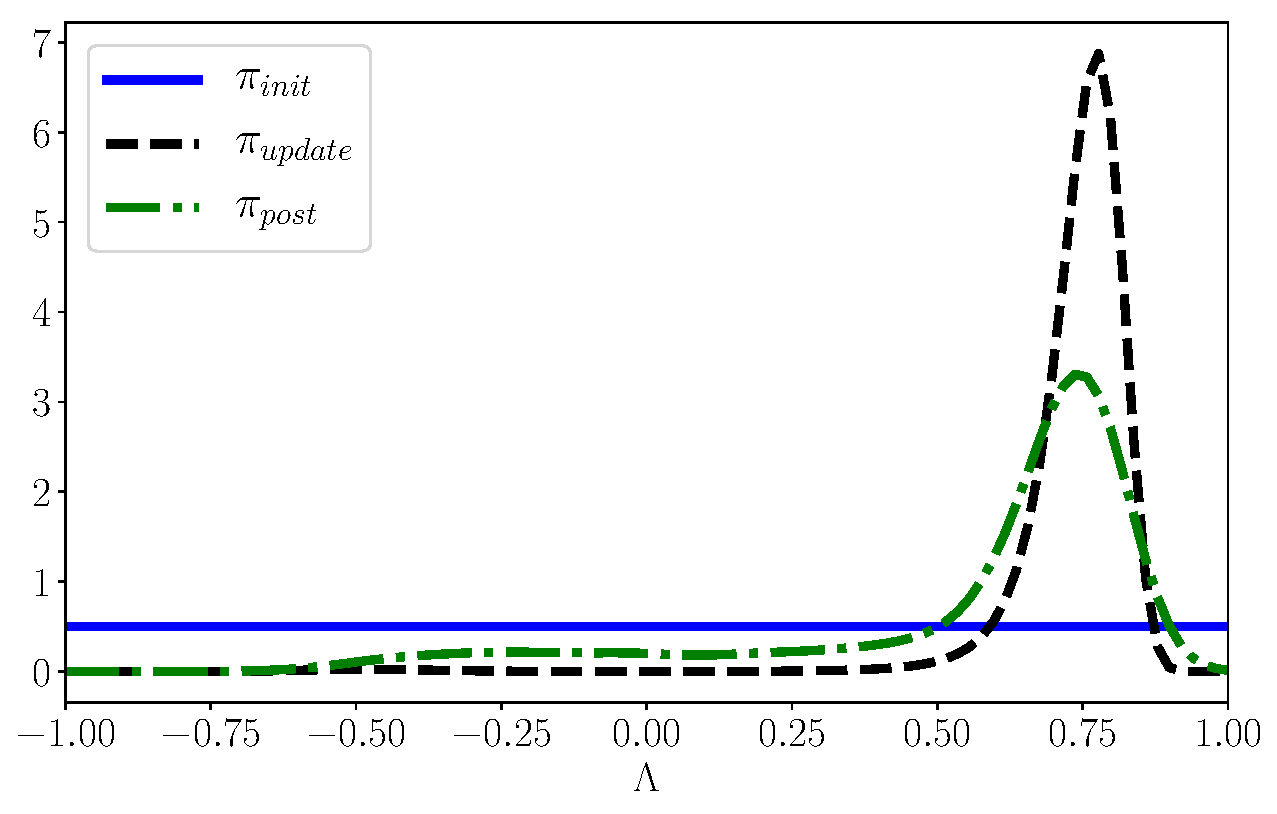
\includegraphics[width=0.49\linewidth]{figures/cbayes_comp_sbayes_50000_paramdens_nonlinear-standalone.pdf}
   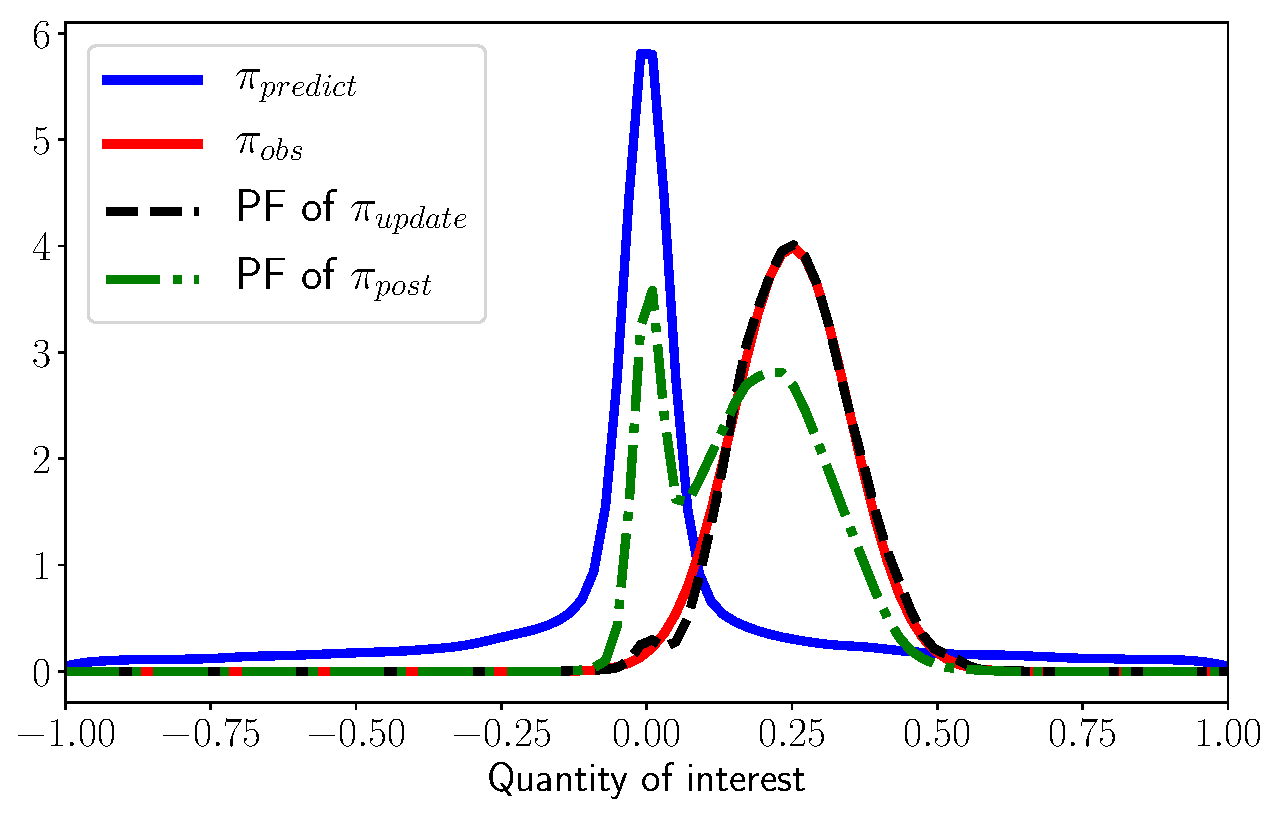
\includegraphics[width=0.49\linewidth]{figures/cbayes_comp_sbayes_50000_outdens_nonlinear-standalone.pdf}
 \caption{(Left) The initial/prior PDF $\initial$ (blue solid curve), updated PDF $\updated$ (black dashed curve), and posterior PDF $\pi_\text{post}$ (green dashed-dotted curve) on $\Lambda$.
 (Right) The push-forward (PF) of the initial/prior PDF $\predicted$ (blue solid curve), observed/likelihood PDF (red solid curve), PF of the updated PDF $\updated$ (black dashed curve), and the PF of the posterior PDF $\pi_\text{post}$ (green dashed-dotted curve) for the QoI.}
 \label{fig:bayes-comparison}
\end{figure}

The takeaway to the above discussion and example is that each density is solving a {\em different} inverse problem.
The posterior density is intended to provide point estimates of a true parameter value whereas the updated density is intended to quantitatively characterize natural variations in parameter values.

Suppose we reformulated this example slightly to make the role of data more central.
Specifically, suppose $Q(\paramref)=0.25$ and noisy measurement data are drawn from a $N(0.25,0.1^2)$, i.e., we assume that $d=Q(\paramref)+\xi$ where $\xi\sim N(0,0.1^2)$.
For the SIP, we could use the sample mean and variance of this data to estimate the ``exact'' observed $N(0.25,0.1^2)$ distribution whereas the data-likelihood would involve a product of normal densities.
In this case, the objective is to use the posterior or updated density to produce an estimate of $\paramref$.
In the next section, we motivate the use of the maximal updated density point as a means of providing a useful point estimate to parameters.


%A critical component in the Bayesian framework is the prior density, which encodes any knowledge or assumptions about them input (parameter) space that we may wish to impose before any data are observed.
%In some cases, the prior and initial densities may be both specified and interpreted identically.
%However, in the Bayesian framework, the impact of the prior on the posterior density is perhaps best understood as a regularization term that makes the inverse problem well--posed by penalizing parameters uninformed by the data.
%Ideally, the prior should not interfere with well--informed parameters, i.e., parameters informed by the data.
%{Unfortunately, well--informed parameters are not known a priori and none of the existing prior elicitation approaches avoid polluting data--informed directions in the parameter space.}






